\documentclass{minimal}
\usepackage{tikz}
\usetikzlibrary{graphs,decorations.pathmorphing,decorations.markings} 
\usetikzlibrary{arrows}
\usepackage{tikz-cd}
\usepackage{amsmath,amssymb}
\usetikzlibrary{arrows,positioning} 

\tikzset{degil/.style={
            decoration={markings,
            mark= at position 0.5 with {
                  \node[transform shape] (tempnode) {$\backslash$};
                  }
              },
              postaction={decorate}
}
}


\begin{document}
\begin{center}
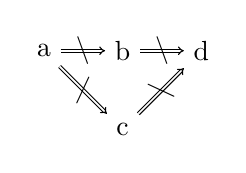
\begin{tikzpicture}[>=stealth,>=implies]
 \graph  {
  a ->[double,degil] {b,c} ->[double,degil] d
};
\end{tikzpicture}

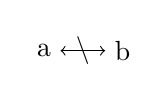
\begin{tikzpicture}[>=stealth,>=implies]
 \graph  {
  a ->[-to,degil] {b} ->[-to] a
};
\end{tikzpicture}
\end{center}


\ \\
\begin{center}
\begin{tikzcd}[arrows=Rightarrow]
   A \arrow[out=30,in=150,degil]{r}{}\arrow[degil]{d} & B \arrow[out=210,in=330]{l}{}\arrow{d}  \\
   E  \arrow{r}{} & F
\end{tikzcd}
\end{center}

\ \\

\begin{center}
\begin{tikzcd}[row sep=huge]
A \arrow[r,"\phi_n"] \arrow[d,swap,"\pi"] &
A_n \arrow[r,"\epsilon_{i,n}"] \arrow[dl,swap,"\psi_n"] \arrow[dr,"\pi_n"] &
M_{n_k}(\mathbb{C}) \arrow[d,"\eta_{i,n}"]
\\
B(H) & & B(H_n) \arrow[ll,dashed]
\end{tikzcd}
\end{center}

\ \\

\begin{center}
\begin{tikzcd}
A \arrow[shift left=1.5ex]{r}{}  & B \arrow[degil]{l}{} \arrow[shift left=1.5ex]{r}{} & C \arrow[degil]{l}{} \\
& D 
\end{tikzcd}
\end{center}

\ \\

\begin{center}
	\begin{tikzcd}[column sep=tiny]
& \pi_1(U_1) \ar[dr] \ar[drr, "j_1", bend left=20]
&
&[1.5em] \\
\pi \ar[ur, "i_1"] \ar[dr, "i_2"']
&
& \pi_1(U_1) \ast_{ \pi } \pi_1(U_2) \ar[r, dashed, "\simeq"]
& \pi_1(X) \\
& \pi_1(U_2) \ar[ur]\ar[urr, "j_2"', bend right=20]
&
&
\end{tikzcd}
\end{center}

\ \\

\begin{center}
\begin{tikzcd}[row sep=huge,column sep=huge]
\text{piandao-lianxu} \arrow[r,shift left=1.5ex] & \text{kewei} \arrow[r,shift left=1.5ex]\arrow[d,shift left=1.5ex]\arrow[l,degil] & \text{lianxu} \arrow[d,,shift left=1.5ex]\arrow[l,degil]\arrow[ld,degil] \\
& \text{youpiandao} \arrow[u]\arrow[r,shift left=1.5ex,degil]\arrow[ru,shift left=1.5ex,degil] & \text{youjixian} \arrow[u,degil]\arrow[l,degil]
\end{tikzcd}
\end{center}

\ \\

\begin{center}
\begin{tikzcd}[arrows=to]
   A \arrow[out=30,in=150,degil]{r}{} & B \arrow[out=210,in=330]{l}{}
\end{tikzcd}
\end{center}

\ \\

\begin{center}
\begin{tikzcd}[arrows=to]
   A \arrow[out=30,in=150]{r}{} & B \arrow[out=210,in=330]{l}{} \arrow[out=30,in=150]{r}{} & E \arrow[out=210,in=330,degil]{l}{} \arrow[out=30,in=150]{r}{} & F \arrow[out=210,in=330,degil]{l}{}
\end{tikzcd}\\
\end{center}

\ \\

\tikzset{
    %Define standard arrow tip
    >=stealth',
    %Define style for boxes
    punkt/.style={
           rectangle,
           rounded corners,
           draw=black, very thick,
           text width=6.5em,
           minimum height=2em,
           text centered},
    % Define arrow style
    pil/.style={
           ->,
           thick,
           shorten <=2pt,
           shorten >=2pt,}
}
\begin{center}
	\begin{tikzpicture}[node distance=1cm, auto,]
 %nodes
 \node[punkt] (market) {Market (b)};
 \node[punkt, inner sep=5pt,below=0.5cm of market]
 (formidler) {Intermediaries (c)};
 % We make a dummy figure to make everything look nice.
 \node[above=of market] (dummy) {};
 \node[right=of dummy] (t) {Ultimate borrower}
   edge[pil,bend left=45] (market.east) % edges are used to connect two nodes
   edge[pil, bend left=45] (formidler.east); % .east since we want
                                             % consistent style
 \node[left=of dummy] (g) {Ultimate lender}
   edge[pil, bend right=45] (market.west)
   edge[pil, bend right=45] (formidler.west)
   edge[pil,<->, bend left=45] node[auto] {Direct (a)} (t);
\end{tikzpicture}
\end{center}
\end{document}